\section{Introduction}


Language agents based on large language models (LLMs) have been developed for a variety of applications~\citep{githubcopilot,brynjolfsson2023generative}, following recent breakthroughs in improving LLMs~\citep{achiam2023gpt,ouyang2022training,team2023gemini}. However, despite their impressive zero-shot performance, LLMs still need to adapt and personalize to a given user and task~\citep{mysore2023pearl,li2023automatic}. In many applications, a natural feedback for LLM-based agents is user edits, where a user queries the agent and edits the agent's response before their own final use. In contrast, typical feedback used for fine-tuning, such as the comparison-based preference feedback in RLHF, is explicitly collected by providing annotators with model responses and asking them to rank~\citep[inter alia]{Ziegler2019FineTuningLM,Stiennon2020LearningTS,Nakano2021WebGPTBQ,Ouyang2022TrainingLM}, making such feedback an expensive choice for improving alignment. Motivated by this observation, we focus on interactive learning of LLM-based language agents using user edits as feedback.\looseness=-1



\begin{figure*}[!t]
    \centering
    \vspace{-10pt}
    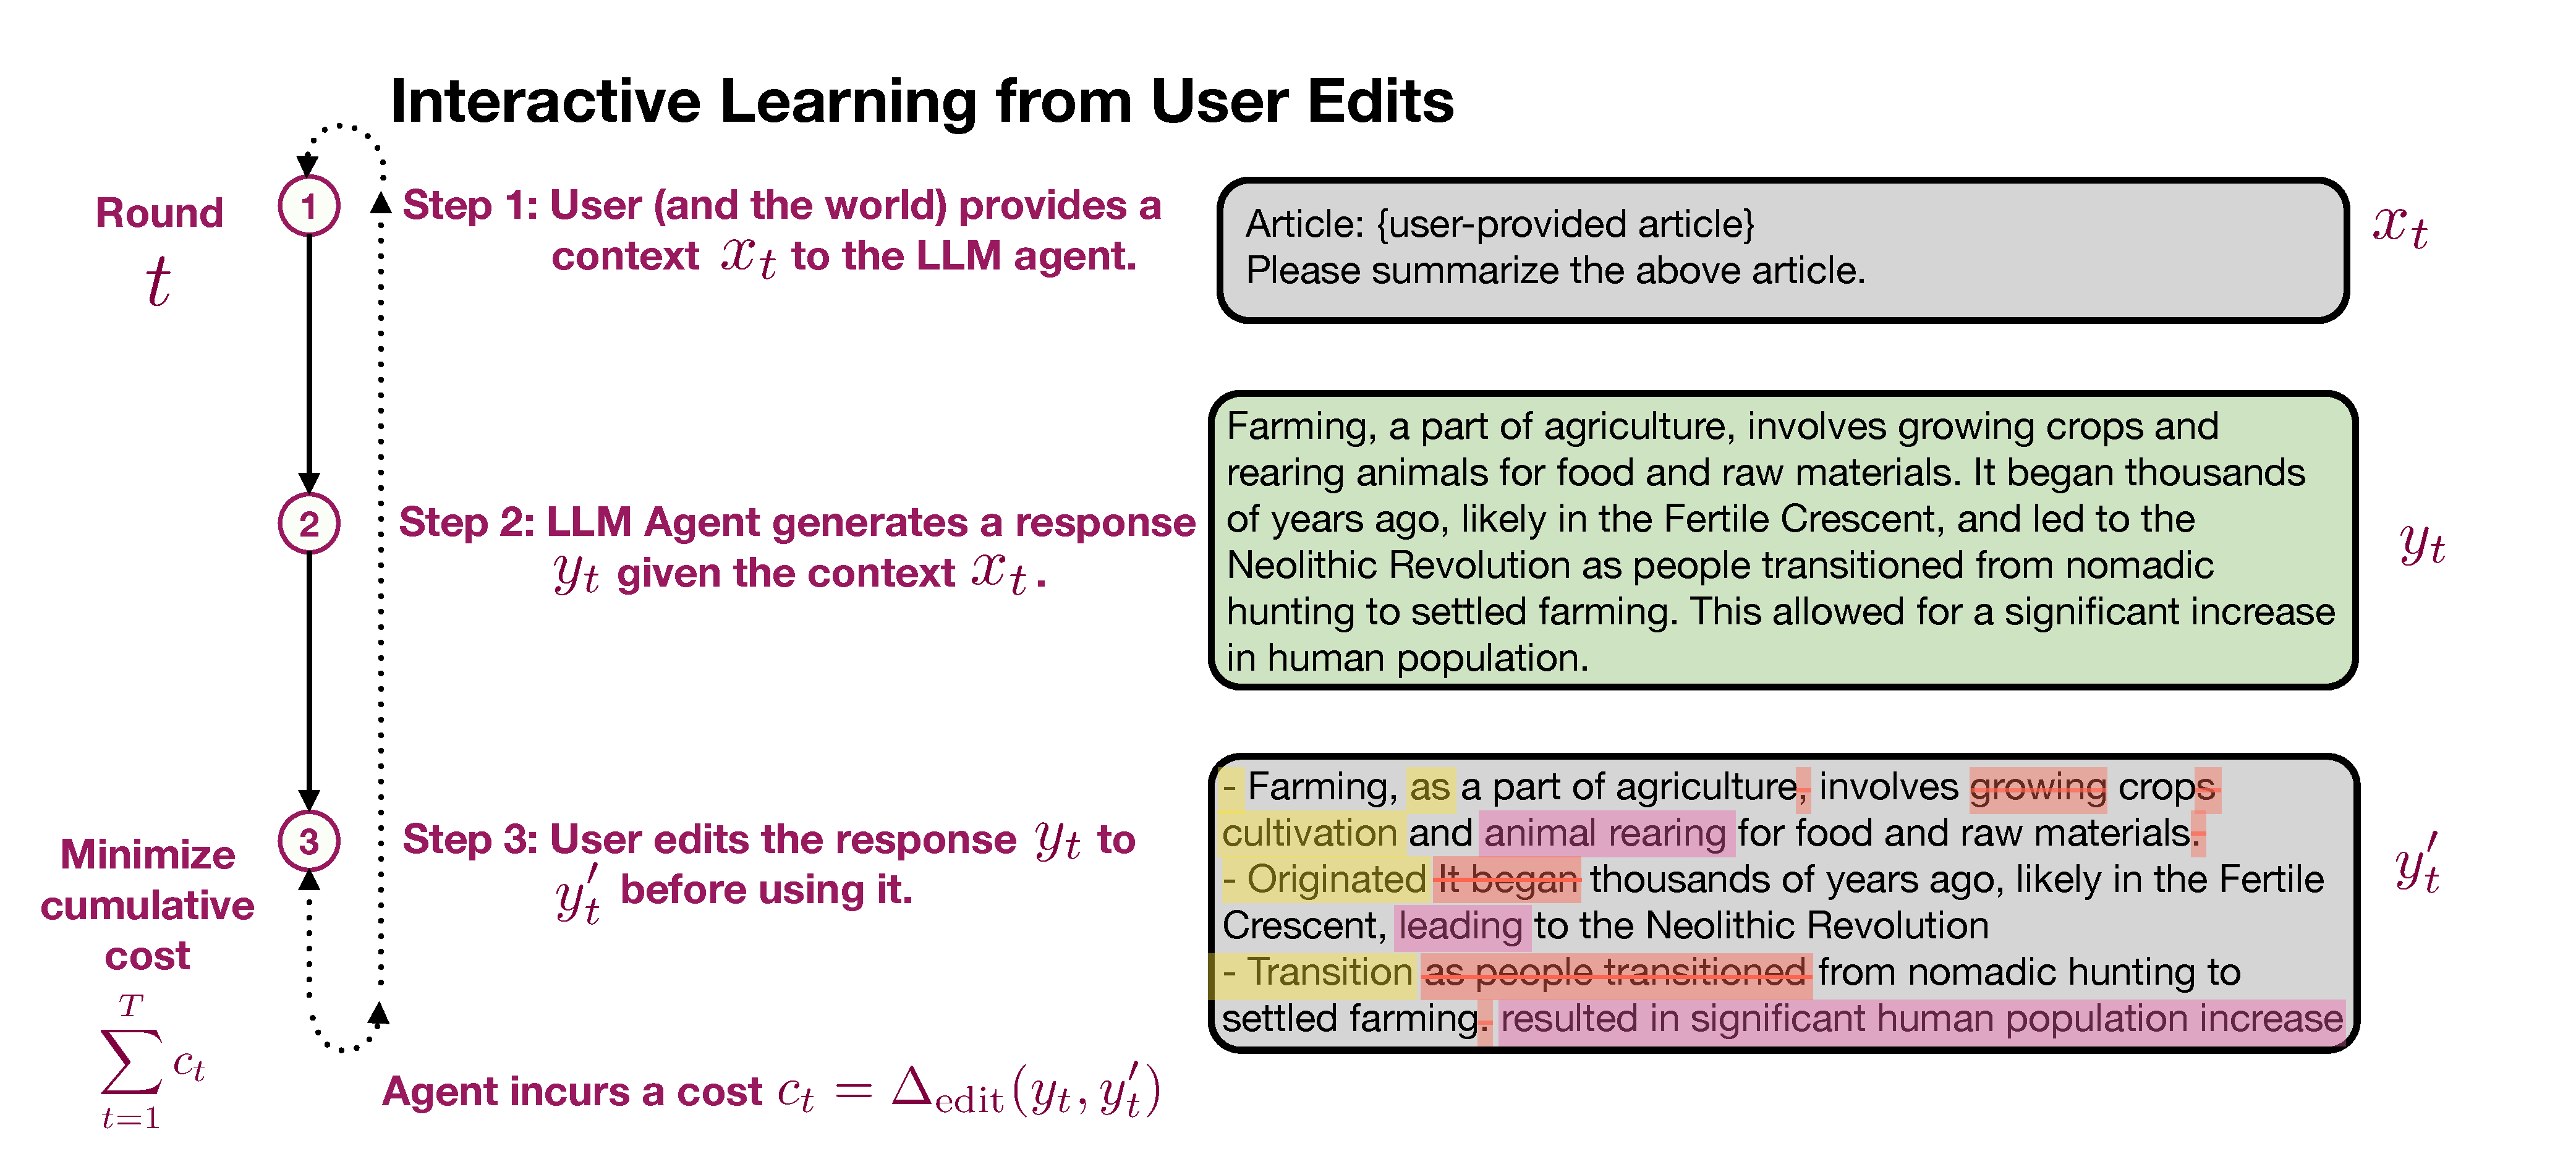
\includegraphics[clip, trim=1cm 0.5cm 3.5cm 1cm, width=1.00\textwidth]{graphs/main_diagram_vertical.pdf} 
    \caption{Illustration of interactive learning from user edits. Color coding in edits is for visualization only -- our agent takes the plain revised text as feedback. }
    \label{fig:main}
    \vspace{-15pt}
\end{figure*}

Consider the scenario in~\pref{fig:main} where a user interacts with an LLM-based writing assistant (agent) to complete their task. The interaction starts with the user (and the world) providing a context to the agent. This context may include a query prompt provided by the user, along with additional information provided by the world, such as the content on the screen, current time, and the user's calendar information. The agent generates a textual response to the user given the context.

In the beginning, the agent's response may not be optimal for the user, as it is not personalized to this user's individual needs and preference. As most users are not familiar with prompt engineering, and LLMs are often able to generate an acceptable response for the task, therefore, users may find it the most convenient to simply edit the response when it is not ideal to suit their needs, rather than trying different prompts to get new responses. The example in~\pref{fig:main} illustrates that the user directly edits the summary generated by the agent to satisfy their preference on bullet point format. It takes time and efforts for the user to make edits. We can measure such cost using a variety of metrics, such as the edit distance between the agent-generated response and the user-revised text. Zero edit from the user is also a useful feedback, reflecting that the agent's response satisfies this user's needs. One important feature of our setting is that \emph{every natural use of the agent yields an edit feedback for learning}. Since there is no distinction between training and testing in this setting, we care about minimizing the user's efforts across all rounds of interaction with the agent.
In summary, our goal is to learn from the implicit feedback in user edit history to minimize the cumulative cost of the user's efforts.\looseness=-1

We conjecture that user edits are driven by user's hidden preference which can be described in natural language. These \emph{preference descriptions} are different from the notion of comparison-based preference used in RLHF. In this paper, we use the word \emph{preference} to mean \emph{preference descriptions}. For instance, preference of the user in~\pref{fig:main} can be described as \emph{bullet points}. In practice, user preference can be compound, such as preferring \emph{bullet point, informal, with emojis} at the same time, and also context-dependent, e.g., \emph{informal} tone when writing an email to a family member, and \emph{formal} tone when writing to a colleague. In more complex settings, user preference can evolve with time (non-stationary), or depend on information unavailable in the context (partially observed). Such user preference may not be fully derivable from the context, and the user may not even be fully aware of all their preference. These considerations imply that user preference is \emph{latent} to the language agent. If the agent could learn the \emph{latent} preference correctly, it can significantly improve its performance by generating satisfactory responses accordingly. Furthermore, preference learned by the agent can be shown to the user to enhance \emph{interpretability}, and can even be modified by the user to improve correctness. Motivated by this, we propose a learning framework, \textbf{\framework} (\textbf{PRE}ference \textbf{L}earning from \textbf{U}ser's \textbf{D}irect \textbf{E}dits), where we seek to learn a textual description of the user preference for a given context using the history of user edits.

In a typical real-world scenario such as writing assistants, one has to potentially update the LLM-based agent for every user. Efficient approaches, therefore, must scale with the number of users. This makes approaches that perform a full fine-tuning of the LLM used by the agent very hard to scale. Furthermore, LLMs typically undergo evaluation on a variety of metrics before being released, and thus fine-tuning them often results in breaking the generalization guarantees offered by these tests. For example, fine-tuning GPT-4 for millions of users can quickly turn very expensive. Approaches such as adding LORA and Adapter layers and only updating them, or using federated learning, can reduce the expense to some extent, while the loss of generalizable alignment remains as a concern. In this work, we focus on leveraging a frozen, black-box LLM, and instead learning a \emph{prompt policy} that can infer textual description of user's preference for a given context, and then use it to directly drive the response generation.

We introduce a simple yet effective algorithm~\textbf{\algname}~(\textbf{C}onsolidates \textbf{I}nduced \textbf{P}references based on \textbf{H}istorical \textbf{E}dits with \textbf{R}etrieval) under the \framework~framework. For a given context,~\algname~first retrieves the $k$-closest contexts from history, and aggregates inferred preferences for these $k$ contexts. It relies on this aggregate preference to generate a response for the given context. If the user performs no edits, then it saves this aggregate preference as the correct preference for the given context. Otherwise, it queries the LLM to infer a plausible preference that explains these user edits made to the agent response, and saves this inferred preference as the correct preference for the given context. A key advantage of~\algname~is that it typically leads to significantly shorter prompts compared to other retrieval methods that use the entire documents or context, as inferred preferences are much shorter than retrieved documents or contexts. This results in a significant reduction in the computational expense of querying the LLM.

We introduce two interactive environments for evaluation, inspired by writing assistant applications. In the first environment, we evaluate the agent's ability to summarize a given document (articles from different sources). In the second environment, we evaluate the agent's ability to compose an email using content from a given document (notes for various purpose). In both tasks, we simulate a GPT-4 user that can generate edits based on a pre-designed \emph{latent} preference. We use documents from several existing domains as our user-provided context, and vary the GPT-4 user's preference based on the domain, in order to capture the real-world context-dependent nature of human user's preference. We evaluate \algname~against several baselines, including approaches that learn context-agnostic user preferences, and retrieval-based approaches that do not learn preferences but directly use past user edits for generation. We show that for both tasks, \algname~achieves the lowest user edit cost compared to baselines, and significantly reduces the cumulative cost compared to using the frozen base agent. Additionally, \algname~results in a lower LLM query cost than other retrieval-based baselines.
Finally, we qualitatively and quantitatively analyze preferences learned by our agents, and find that they show significant similarity to the ground truth latent preferences in our setup.













